%\title{emnlp 2017 instructions}
% File emnlp2017.tex
%

\documentclass[11pt,letterpaper]{article}
\usepackage{emnlp2017}
\usepackage{times}
\usepackage{latexsym}
\usepackage{graphicx}
\usepackage{booktabs}
\usepackage{color}


% Uncomment this line for the final submission:
%\emnlpfinalcopy

%  Enter the EMNLP Paper ID here:
\def\emnlppaperid{***}

% To expand the titlebox for more authors, uncomment
% below and set accordingly.
% \addtolength\titlebox{.5in}    

\newcommand\BibTeX{B{\sc ib}\TeX}


%\title{Including lexical morphosyntactic information\\in a neural PoS tagging architecture}
\title{Improving neural tagging with lexical information}

% Author information can be set in various styles:
% For several authors from the same institution:
% \author{Author 1 \and ... \and Author n \\
%         Address line \\ ... \\ Address line}
% if the names do not fit well on one line use
%         Author 1 \\ {\bf Author 2} \\ ... \\ {\bf Author n} \\
% For authors from different institutions:
% \author{Author 1 \\ Address line \\  ... \\ Address line
%         \And  ... \And
%         Author n \\ Address line \\ ... \\ Address line}
% To start a seperate ``row'' of authors use \AND, as in
% \author{Author 1 \\ Address line \\  ... \\ Address line
%         \AND
%         Author 2 \\ Address line \\ ... \\ Address line \And
%         Author 3 \\ Address line \\ ... \\ Address line}
% If the title and author information does not fit in the area allocated,
% place \setlength\titlebox{<new height>} right after
% at the top, where <new height> can be something larger than 2.25in
%\author{Siddharth Patwardhan \and Preethi Raghavan \\
%  {\tt publication@emnlp2017.net}}
\author{Anonymous submission}

\date{}
\hypersetup{draft}
\begin{document}

\maketitle

\begin{abstract}
  Neural part-of-speech tagging has achieved competitive results with the incorporation of character-based and
  pre-trained word embeddings. In this paper, we show that a state-of-the-art bi-LSTM tagger can benefit from using
  information from morphosyntactic lexicons as additional input. The tagger, trained on several dozen languages, shows a
  consistent, average improvement of 2.6\% tagging accuracy for systems without character-based embeddings, and an
  improvement of 0.6\% in the presence of character-based embeddings, which indicates that morphosyntactic lexicons do
  indeed provide information that is not captured by the embeddings themselves, both character-based and word-level. The
  improvements are particularly important for the smaller datasets.
\end{abstract}


\section{Introduction}

Part-of-speech tagging is now a classic task in natural language processing, for which many systems have been developed
or adapted for a large variety of languages. Its aim is to associate each ``word'' with a morphosyntactic tag, whose
granularity can range from a simple morphosyntactic category, or part-of-speech (hereafter PoS), to finer categories
enriched with morphological features (gender, number, case, tense, mood, etc.).

The use of machine learning algorithms trained on manually annotated corpora has long become the standard way to develop
PoS taggers. A large variety of algorithms have been used, such as (in approximative chronological order) bigram and
trigram hidden Markov models \cite{merialdo94,brants96,brants00}, decision trees \cite{schmid94,magerman95}, maximum
entropy Markov models (MEMMs) \cite{ratnaparkhi96} and Conditional Random Fields (CRFs)
\cite{lafferty01,constant12}. Recently, neural approaches have reached very competitive accuracy levels, improving over
the state of the art in an number of settings \cite{plank16}.

As a complement to  annotated training corpora, external lexicons can be a valuable source of information.
First, morphosyntactic lexicons provide a large inventory of (word,~PoS)
pairs. Such lexical information can be used in the form of constraints at tagging time \cite{kim99,hajic00tagging} or
during the training process as additional features combined with standard features extracted from the training corpus
\cite{chrupala08,goldberg09,denis12}.

Second, lexical information encoded in vector representations, known as word embeddings, have emerged more
recently \cite{bengio03,collobert08,chrupala13,ling15,ballesteros15,muller15}. Such representations, often
extracted from large amounts of raw text, have proved very useful for numerous tasks including PoS tagging, in
particular when used in recurrent neural networks (RNNs) and more specifically in mono- or bi-directional, word-level or
character-level long short-term memory networks (LSTMs) \cite{hochreiter97,ling15,ballesteros15,plank16}.

Character-level embeddings are of particular interest for PoS tagging as they generate vector representations that
result from the internal character-level make-up of each word. It can generalise over relevant sub-parts such as
prefixes or suffixes, thus directly addressing the problem of unknown words. However, unknown words do not always follow
such generalisations. In such cases, character-level models cannot bring any advantage. This is a difference with
external lexicons, which provides information about any word it contains, yet without any quantitative distinction
between relevant and less relevant information.

Therefore, a comparative assessment of the advantages of using character-level embeddings and external lexical
information is an interesting idea to follow. However, the inclusion of morphosyntactic information from lexicons
into neural PoS tagging architecture, as a replacement or complement to character-based or pre-computed word embeddings,
remains to be investigated. In this paper, we describe how such an inclusion can be achieved and show, based on
experiments on corpora from the Universal Dependencies repository (version 1.3), that it leads to significant
improvements over \citeauthor{plank16}'s (\citeyear{plank16}) state-of-the-art results.

%\textcolor{blue}{Moreover, lexicon information is qualitatively different from word and character embedding information in that it improves the prediction of A CERTAIN CLASS OF WORDS}

\section{Baseline bi-LSTM tagger}
\label{sec:baselinearchitecture}
As shown by \citet{plank16}, state-of-the-art performance can be achieved using a bi-LSTM architecture fed with word
representations. Optimal performance is achieved representing words using the concatenation of (i) a word vector
$\vec{w}$ built using a word embedding layer, called its {\em word embedding}, and (ii) a representation $\vec{c}$ of
the word's characters, called its {\em character-based embedding} built using a character-level bi-LSTM, which is
trained jointly with the word-level layers. Further improvements can be obtained on most but not all languages by
initialising the word embedding layer with pre-computed word embeddings. We refer to \citet{plank16} for further details.

\section{Integrating lexical information}

We extend this bi-LSTM architecture with an additional input layer that
contains token-wise features obtained from a lexicon. The input vector $\vec{l}$ for a given word is an $n$-hot vector
where each active value corresponds to one of the possible labels in the lexicon. For instance, the English word
\textit{house}, which is both a singular noun and a verb in its base form, will be associated to a 2-hot input
vector.  Note that this way of incorporating lexicon information as new features in an input layer is label-set
agnostic, and no explicit relation is needed between the morphosyntactic inventory of the lexicon and the label set we
are aiming at predicting, namely the 17-label UD tagset.

Figure~\ref{fig:schema} shows how the output of this input layer is concatenated to that of the two baseline input
layers, namely the word embedding $\vec{w}$ and (if enabled) the character-based embedding $\vec{c}$. The result of this
concatenation serves as an input to the bi-LSTM layer.

% We do not use the option of multitask learning of the tagger presented by \citeauthor{plank16}'s
% (\citeyear{plank16}), and we use a single bi-LSTM layer instead of multi-layer stacking. While such systems can
% improve the overall results,\footnote{Note however that \citeauthor{plank16}'s (\citeyear{plank16})
%     secondary task---predicting the frequency class of each word---results in better OOV scores but virtually identical
%     overall scores when averaged over all tested languages/corpora.} our goal is to clearly assess the relative
% contribution of information provided by an external morphosyntactic lexicon in contrast to word and character embeddings
% on an already very competitive single-layer baseline.

\begin{figure}
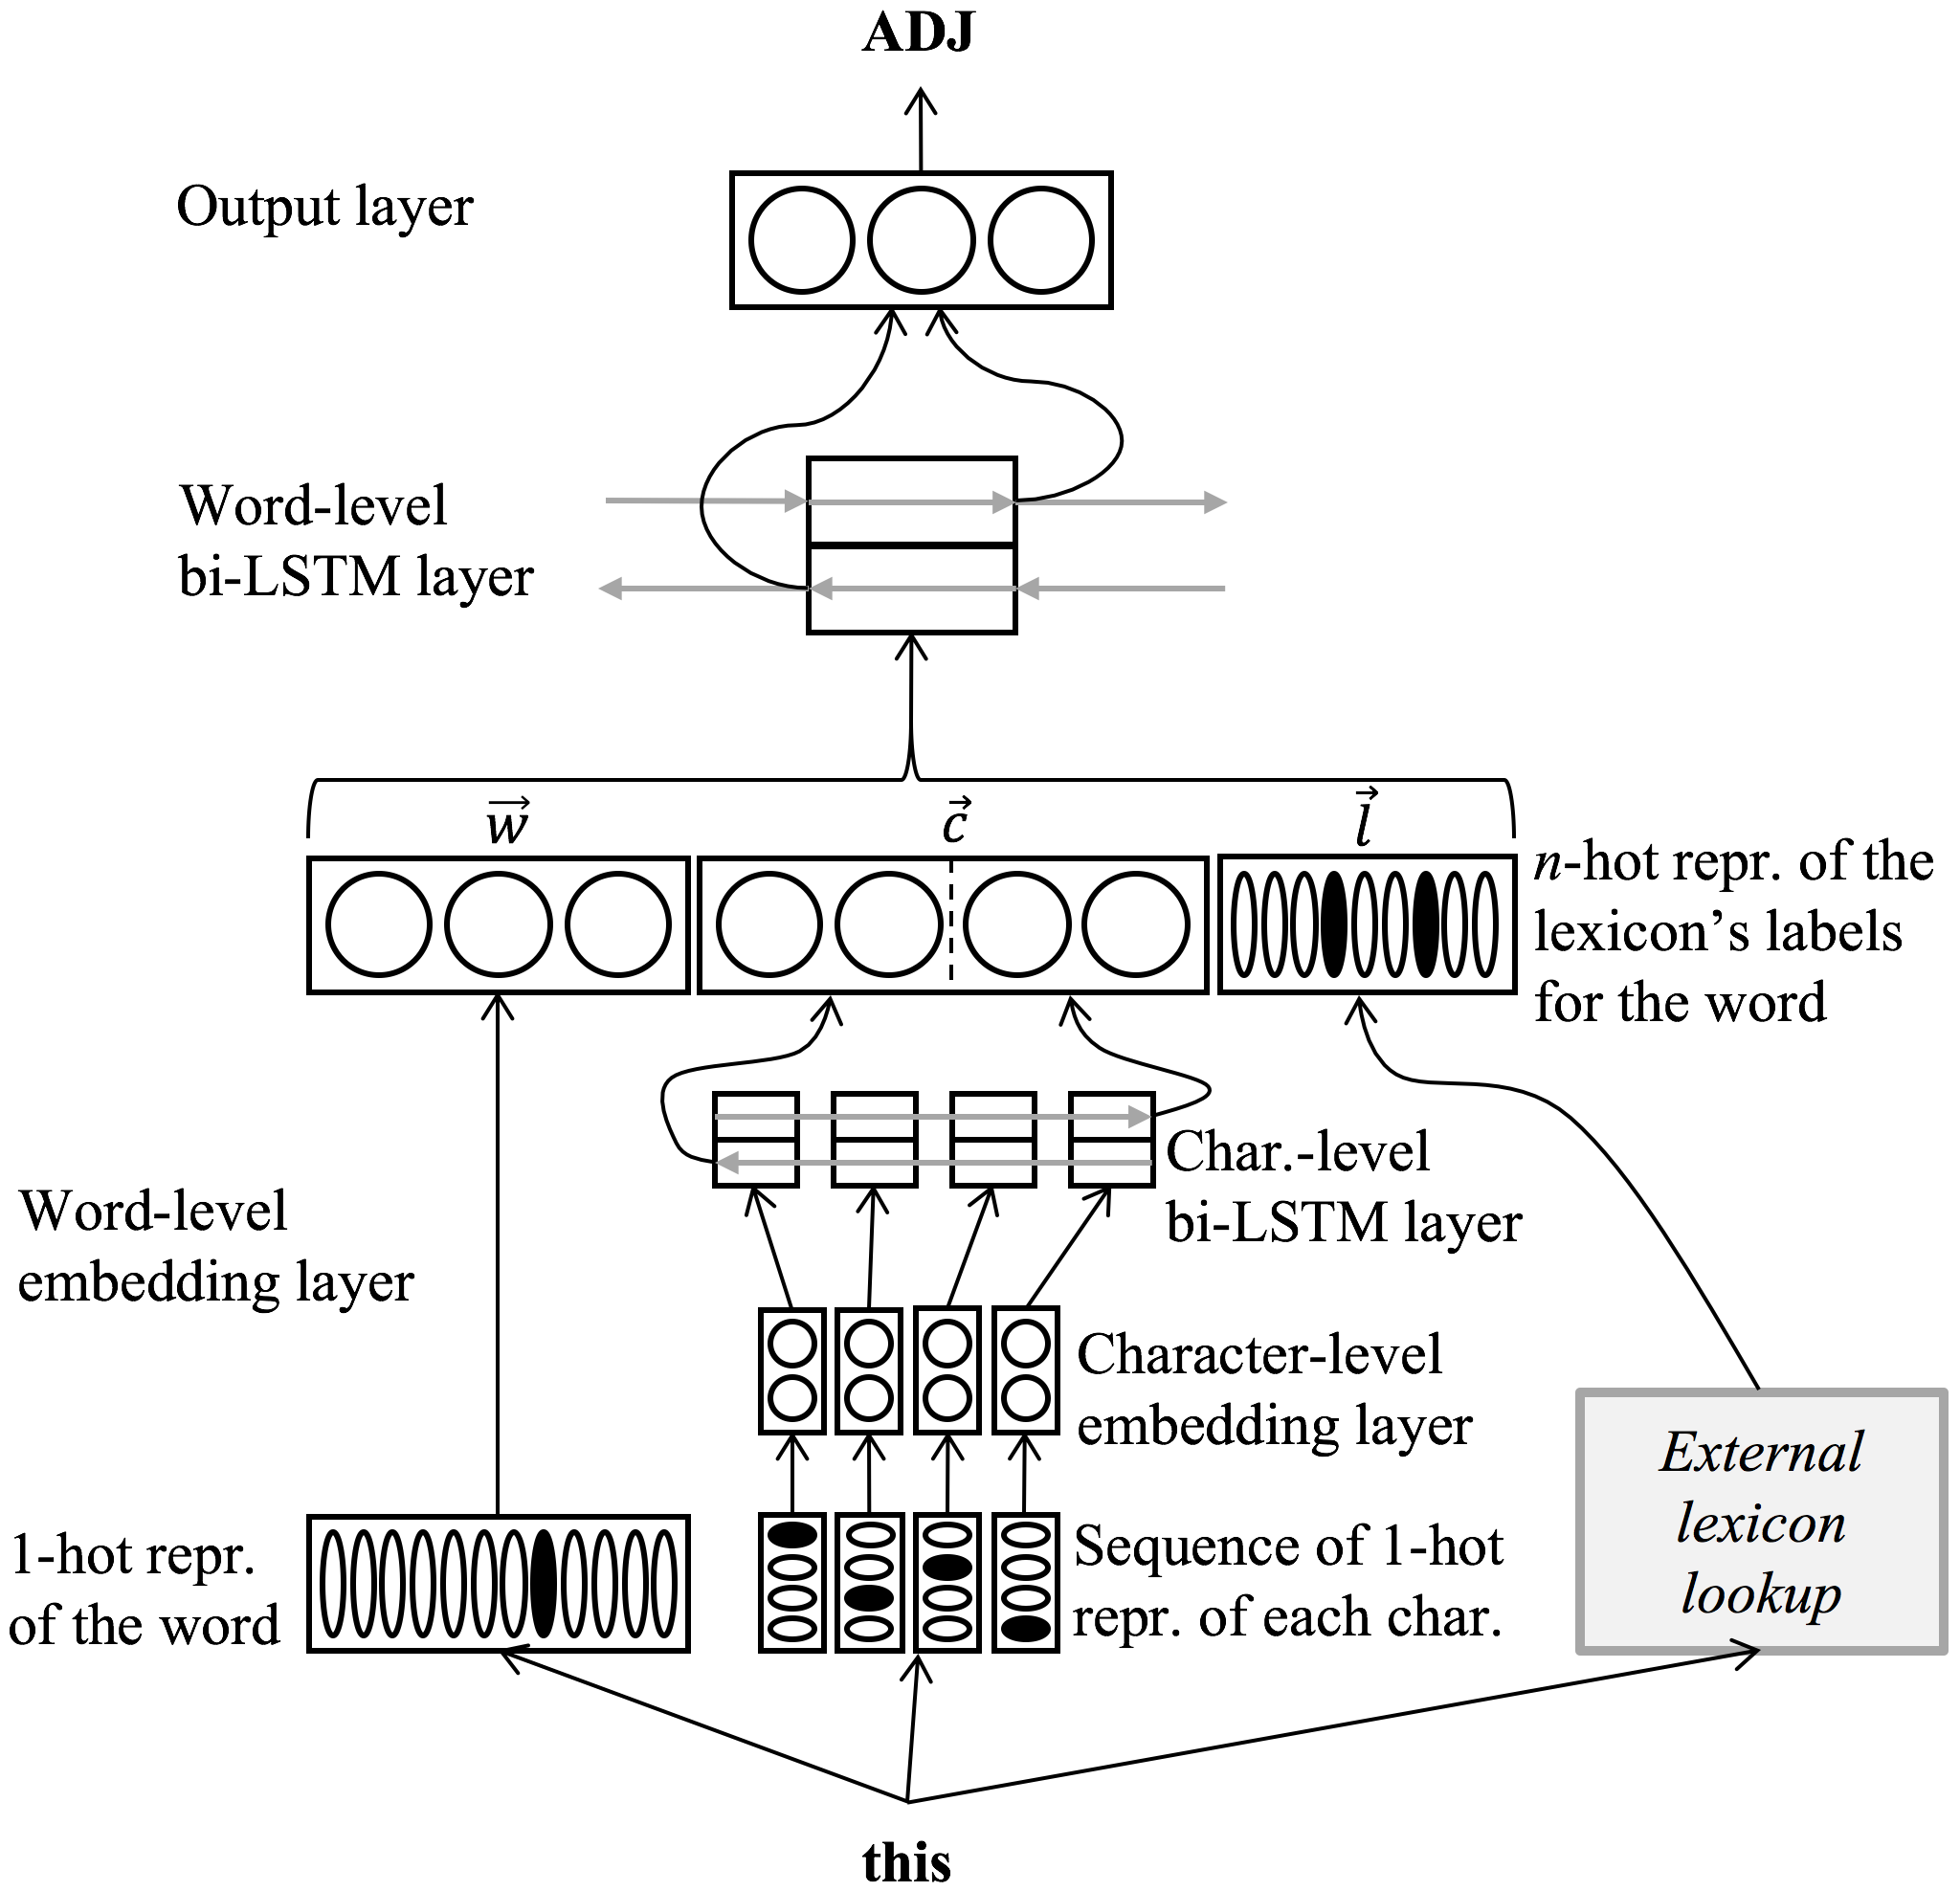
\includegraphics[width=\columnwidth]{emnlp17schemaB2}
%\caption{Schematic representation of the architecture of (a)~\citeauthor{plank16}'s (\citeyear{plank16}) bi-LSTM tagger,
%and (b)~our extension thereof for integrating external morphosyntactic lexical information. Each of these two schemas
%concerns a single word. Connections of the word-level LSTM cells to their counterparts for the preceeding and
%following word are represented with grey arrows.}\label{fig:schema}
\caption{Schema of our extension of \citeauthor{plank16}'s (\citeyear{plank16})
  bi-LSTM tagging architecture for integrating external morphosyntactic lexical information. This schema concerns a
  single word, here ``this.'' Connections of the word-level LSTM cell to its counterparts for the preceeding and
  following word are represented with grey arrows.}\label{fig:schema}
\end{figure}

%\section{Experiments}

\section{Data}

We use the Universal Dependencies (UD) datasets for our experiments. However, as the test data of UD 2.0 was not
available at the time of the submission, we performed our experiments on a previous version of this corpus
collection. More precisely, in order to facilitate comparison with \citeauthor{plank16}'s (\citeyear{plank16}), we
performed all experiments on the version 1.3 of UD \cite{ud13}.

We used two types of lexical information sources, thereby obtaining one to three lexicons for each language, in the way
sketched below. We trained our tagger with and without character-based embeddings, and with or without Polyglot-based
initialisation (when available), both without lexical information and with lexicon information from all available
lexicons, resulting in 4 to 12 training configurations. We determine the best performing lexicon for each language based
on tagging accuracy on the development set. In the remainder of this paper, all information about the lexicons
(Table~\ref{tbl:lex}) and accuracy results are restricted to these best performing lexicons.

The sources of lexical information we used are twofold. The first one is the
Apertium\footnote{https://svn.code.sf.net/p/apertium/svn/languages} and the
Giellatekno\footnote{https://victorio.uit.no/langtech/trunk/langs} projects. For languages for which an Apertium
morphological lexicon is available, this lexicon was used. For other languages, we downloaded from the OPUS corpus
collection the corresponding monolingual part of OpenSubtitles2016, tokenised it, extracted the 1 million most frequent
tokens, and retrieved all their morphological analyser by the Apertium morphological transducer---or by the Giellatekno
morphological transducer when none was available from Apertium. All these analyses were then gathered in the form of a
lexicon. In a second step, we converted all lexicons obtained using manually crafted rules, so that each lexical entry
contains a (inflected) wordform, a lemma, a PoS from the Universal PoS
tagset,\footnote{http://universaldependencies.org/u/pos/all.html} and a set of attribute-value pairs from the Universal
Features.\footnote{http://universaldependencies.org/u/feat/all.html} We then created two variants of the lexicons
obtained: a {\em full} variant in which labels are universal PoS, and a {\em coarse} variant in which labels are the
concatenation of the universal PoS and morphological feature-value pairs.

We also took advantage of other existing lexicons. For space reasons, we are not able to describe here the language-specific
transformations we applied to some of these lexicons. See Table~\ref{tbl:lex} and its caption for more information.


Finally, whenever available and following \citet{plank16}, we performed experiments using Polyglot pre-computed
embeddings \cite{alrfou13}. Languages for which Polyglot embeddings are available are indicated in Table~\ref{tbl:lex}.

\addtocounter{footnote}{-1}

%\begin{table*}
%\centering
%\scriptsize
%\begin{tabular}{l|lrr|llrrc}
%\toprule
%Lang. & \multicolumn{3}{c}{\sc lex} & \multicolumn{3}{|c}{\sc lex2} & Polyglot\\
%code & type & \#entries & \#tags (full/coarse) & name & reference & \#entries & \#tags & embeds\\
%\midrule
%ar & {\em ap.lex} & 650,592 & 658/15 &  &  &  &  & yes\\
%bg & {\em ap.lex} & 93,186 & 286/16 & MULTEXT-East V4 & \citep{erjavec10} & 53,056 & 12 & yes\\
%ca & {\em ap.lex} & 369,927 & 188/13 &  &  &  &  & yes\\
%cs & {\em ap.lex} & 1,874,737 & 1119/15 & Morfflex (filtered) & \citep{hajic13} & 2,094,860 & 65 & yes\\
%da & {\em ap.lex} & 683,456 & 164/15 & STO & \citep{braasch08} & 591,035 & 45 & yes\\
%de & {\em ap.lex} & 2,179,689 & 536/16 & DeLex & \citep{sagot14delex} & 465,434 & 52 & yes\\
%el & {\em ap.lex} & 47,131 & 190/12 & DELA\_gr & \citep{symeonidis99} & 1,988,898 & 25 & yes\\
%en & {\em ap.lex} & 126,928 & 108/15 & EnLex & \citep{sagot10lefff} & 490,511 & 47 & yes\\
%es & {\em ap.lex} & 324,517 & 157/12 & Le{\it ff}e & \citep{molinero09} & 755,858 & 34 & yes\\
%et & {\em gt.ma} & 43,553 & 202/12 & MULTEXT-East V4 & \citep{erjavec10} & 133,804 & 11 & yes\\
%eu & {\em ap.lex} & 52,618 & 37/14 &  &  &  &  & yes\\
%fa &  &  &  & PerLex & \citep{sagot10perlex} & 511,840 & 37 & yes\\
%fi & {\em gt.ma} & 227,530 & 202/13 &  &  &  &  & yes\\
%fr & {\em ap.lex} & 136,025 & 135/13 & Le{\it fff} & \citep{sagot10lefff} & 539,278 & 25 & yes\\
%ga &  &  &  & inmdb & \citep{mechura14} & 113,975 & 32 & yes\\
%gl & {\em ap.lex} & 240,698 & 165/13 & LeffGa & \citep{sagot10lefff} & 742,954 & 28 & \\
%grc &  &  &  & Diogenes (Greek) & \citep{heslin07} & 1,313,962 & 18 & \\
%he & {\em ap.lex} & 267,533 & 107/16 &  &  &  &  & yes\\
%hi & {\em ap.lex} & 158,605 & 201/14 &  &  &  &  & yes\\
%hr &  &  &  & HML & \citep{oliver04} & 1,360,687 & 22 & yes\\
%hu & {\em gt.ma} & 2,937 & 4/3 & MULTEXT-East V4 & \citep{erjavec10} & 75,354 & 834 & \\
%id & {\em ap.lex} & 12,199 & 38/14 & Kateglo & \scalebox{0.9}{\url{github.com/ivanlanin/kateglo}} & 72,217 & 118 & yes\\
%it & {\em ap.lex} & 278,356 & 154/14 & Morph it! & \citep{zanchetta05} & 422,756 & 16 & yes\\
%kk & {\em gt.ma} & 434,119 & 1274/16 &  &  &  &  & \\
%la &  &  &  & Diogenes (Latin) & \citep{heslin07} & 562,409 & 16 & \\
%lv & {\em ap.lex} & 313,642 & 583/14 &  &  &  &  & \\
%nl & {\em ap.lex} & 167,302 & 85/14 & Alpino lexicon V1 & \citep{bouma00} & 80,928 & 65 & yes\\
%no & {\em ap.lex} & 2,469,905 & 158/13 & OrdBank & \citep{hagen10} & 880,503 & 224 & yes\\
%pl & {\em ap.lex} & 1,316,112 & 1592/15 & PolLex & \citep{sagot07ltc} & 1,399,697 & 1,082 & yes\\
%pt & {\em ap.lex} & 158,504 & 155/14 & Labellex\_pt & \citep{ranchhod99} & 1,258,205 & 281 & yes\\
%ro & {\em ap.lex} & 229,341 & 247/13 & MULTEXT-East V4 & \citep{erjavec10} & 378,113 & 14 & \\
%ru & {\em ap.lex} & 4,400,935 & 847/16 &  &  &  &  & \\
%sl & {\em ap.lex} & 653,965 & 1110/14 & SloLeks & \citep{krek08} & 957,525 & 25 & yes\\
%sv & {\em ap.lex} & 2,378,232 & 205/12 & Saldo & \citep{borin08} & 1,214,971 & 214 & yes\\
%tr & {\em gt.ma} & 417,340 & 1764/14 &  &  &  &  & \\
%zh & {\em ap.lex} & 7,617 & 14/13 &  &  &  &  & \\
%\bottomrule
%\end{tabular}
%\caption{Information about lexical informations used in this paper.}\label{tbl:lex}
%\end{table*}

\begin{table}[t]
\centering
\scriptsize
\begin{tabular}{llrrr|rr}
\toprule
 & Name & \#entries & \#tags  & cov.& TTR & PG \\
 &  & ($\times 10^3$) &   & (\%)&  &  \\
\midrule 
ar &   Apertium & 651 & 15 & 46 &0.09& yes \\
bg & Multext-East & 53 &12 & 68 & 0.18 & yes \\
ca &  Apertium & 379 & 13 & 80 & 0.06 & yes \\
cs &  Apertium & 1,875 & 15 & 68 & 0.10 & yes \\
da & Apertium & 683 & 15 & 72 & 0.19 & yes \\
de & DeLex & 465 & 52 & 79 & 0.18 &yes\\
el & Apertium & 47 & 12 & 48 & 0.20 & yes \\
en & Apertium & 127 & 12 & 78 & 0.09& yes \\
es & Le{\it ff}e &  756 & 34 & 87 & 0.12 &yes\\
et & GiellateknoMA & 44 & 12 & 52 & 0.23 & yes \\
eu & Apertium\textsubscript{full} & 53 &  14 & 42 & 0.22 &  yes \\
fa  & PerLex &  512 & 37 & 69 & 0.10 & yes\\
fi & GiellateknoMA & 228 & 13 & 54 & 0.29 & yes \\
fr & Le{\it fff} & 539 & 25 & 88 &0.11 &yes\\
ga & inmdb & 114 & 32 & 35 & 0.26& yes\\
gl & Apertium & 241 & 12 & 85  & 0.12 &no\\
grc  & Diogenes & 1,314 & 18 & 46 & 0.20 &no\\
he & Apertium & 268 & 16 & 71 & 0.12 & yes\\
hi & Apertium & 159 & 14 & 83 & 0.05 & yes\\
hr  & HML   & 1,361 & 22 & 85 & 0.21 & yes \\
%hu & GillateknoMA & 3 & 3 & 1 & 0.33 &no \\
id & Apertium\textsubscript{full}& 12 & 38 &61 &0.18 & no   \\
it & Apertium & 278 &14 & 78 & 0.10 & yes\\
kk & ApertiumMA& 434 & 16 &  79 & 0.48 & no\\
la  & Diogenes & 562 & 16 & 83 & 0.31 &no\\
lv & Apertium & 314 & 14  & 58  & 0.33& no \\
nl &  Alpino lexicon  & 81 & 65 & 77 & 0.14&yes\\
no & Apertium & 2,470 & 13 & 66 & 0.11 & yes\\
pl & Apertium & 1,316 &  15 & 61 & 0.31 & yes\\
pt & Apertium & 159 & 155 & 72 & 0.13 & yes\\
ro &  MULTEXT-East  & 378 & 14 & 66 & 0.18 & no \\
ru & Apertium & 4,401 &16& 61 & 0.32 & no  \\
sl & Apertium & 654 & 14 & 70 & 0.24 &yes\\
sv & Saldo & 1,215 & 214 & 88 & 0.17 & yes\\
tr & ApertiumMA & 417 & 14 & 74 & 0.32  &no \\
zh & Apertium & 8 & 13 & 34 & 0.16 & no \\
% ar &   Apertium & 651k & 15 & 45.88\% &0.09& yes \\
% bg & Multext-East & 53k &12 & 67.59\% & 0.18 & yes \\
% ca &  Apertium & 379k & 13 & 80.06\% & 0.06 & yes \\
% cs &  Apertium & 1,875k & 15  & 0.10 & yes \\
% da & Apertium & 683k & 15 & 71.93\% & 0.19 & yes \\
% de & DeLex & 465k & 52 & 78.78\% & 0.18 &yes\\
% el & Apertium & 47k & 12 & 48.22\% & 0.20 & yes \\
% en & Apertium & 127k & 12 & 77.61\% & 0.09& yes \\
% es & Le{\it ff}e &  756K & 34 & 87.02\% & 0.12 &yes\\
% et & GiellateknoMA & 44k & 12 & 51.55\% & 0.23 & yes \\
% eu & Apertium\textsubscript{full} & 53k &  14 & 42.14\% & 0.22 &  yes \\
% fa  & PerLex &  512k & 37 & 69.41\% & 0.10 & yes\\
% fi & GiellateknoMA & 228k & 13 & 53.54\% & 0.29 & yes \\
% fr & Le{\it fff} & 539k & 25 & 87.59\% &0.11 &yes\\
% ga & inmdb & 114k & 32 & 34.57\% & 0.26& yes\\
% gl & Apertium & 241k & 12 & 85.35\%  & 0.12 &no\\
% grc  & Diogenes & 1,314k & 18 & 45.93\% & 0.20 &no\\
% he & Apertium & 268k & 16 & 71.04\% & 0.12 & yes\\
% hi & Apertium & 159k & 14 & 82.87\% & 0.05 & yes\\
% hr  & HML   & 1,361k & 22 & 84.81\% & 0.21 & yes \\
% hu & GillateknoMA & 3k & 3 & 1.11\% & 0.33 &no \\
% id & Apertium\textsubscript{full}& 12k & 38 &61.37\% &0.18 & no   \\
% it & Apertium & 278k &14 & 78.37\% & 0.10 & yes\\
% kk & ApertiumMA& 434k & 16 &  79.06\% & 0.48 & no\\
% la  & Diogenes & 562k & 16 & 83.25\% & 0.31 &no\\
% lv & Apertium & 314k & 14  & 58.05\%  & 0.33& no \\
% nl &  Alpino lexicon  & 81k & 65 & 76.80\% & 0.14&yes\\
% no & Apertium & 2,470k & 13 & 66.16\% & 0.11 & yes\\
% pl & Apertium & 1,316k &  15 & 61.30\% & 0.31 & yes\\
% pt & Apertium & 159k & 155 & 71.63\% & 0.13 & yes\\
% ro &  MULTEXT-East  & 378k & 14 & 66.46\% & 0.18 & no \\
% ru & Apertium & 4,401k &16& 60.85\% & 0.32 & 16  \\
% sl & Apertium & 654k & 14 & 70.00\% & 0.24 &yes\\
% sv & Saldo & 1,215k & 214 & 88.33\% & 0.17 & yes\\
% tr & ApertiumMA & 417k & 14 & 73.60\% & 0.32  &no \\
% zh & Apertium & 8k & 13 & 33.91\% & 0.16 & no \\

\bottomrule
\end{tabular}
\caption{Dataset information. Best per-language lexicon along with its size, number of tags and coverage (``cov.'') over the UD1.3
  corpus. ``MA'' stands for morphological-analyser-based lexicon. Lexicons based on Apertium and Giellatekno
  data are in their {\em coarse} version unless {\em full} is indicated. Other lexicons
  have been adapted from available resources.\footnotemark{} We also provide the type-token ratio of the 
  corpus (TTR) and whether there were available polyglot embeddings (PG) to initialize $\vec{w}$.}\label{tbl:lex}
\end{table}

\footnotetext{\citealp{bouma00,oliver04,heslin07,borin08,molinero09,sagot10lefff,erjavec10,sagot10perlex,mechura14,sagot14delex}.}

\section{Experimental setup}

\begin{table*}[t]
\centering\scriptsize
\begin{tabular}{l|rrr|rrr|rrr}
\toprule
Language & \multicolumn{3}{c}{Baseline} & \multicolumn{3}{c}{With best lexicon} & \multicolumn{3}{c}{Gain when using} \\
 & \multicolumn{3}{c}{(no lexicon)} & \multicolumn{3}{c}{(selected on dev, cf.~Tab.~\ref{tbl:lex})} & \multicolumn{3}{c}{best lexicon} \\
 & \multicolumn{1}{c}{$\vec{w}$} & \multicolumn{1}{c}{$\vec{w}+\vec{c}$} & \multicolumn{1}{c}{$\vec{w}_P+\vec{c}$} & \multicolumn{1}{c}{$\vec{w}$} & \multicolumn{1}{c}{$\vec{w}+\vec{c}$} & \multicolumn{1}{c}{$\vec{w}_P+\vec{c}$} & \multicolumn{1}{c}{$\vec{w}$} & \multicolumn{1}{c}{$\vec{w}+\vec{c}$} & \multicolumn{1}{c}{$\vec{w}_P+\vec{c}$} \\
\midrule
Arabic (ar) & 93.90 & 95.99 & 96.20 & 94.58 & 96.05 & 96.22 & +0.68 & +0.06 & +0.02\\
Bulgarian (bg) & 94.50 & 98.11 & 97.62 & 96.29 & 98.30 & 97.86 & +1.79 & +0.18 & +0.24\\
Catalan (ca) & 96.14 & 98.03 & 98.17 & 97.58 & 98.21 & 98.26 & +1.44 & +0.18 & +0.09\\
Czech (cs) & 95.93 & 98.03 & 98.10 & 96.74 & 98.46 & 98.41 & +0.81 & +0.43 & +0.31\\
Danish (da) & 90.16 & 95.41 & 95.62 & 94.20 & 96.24 & 96.14 & +4.04 & +0.83 & +0.53\\
German (de) & 87.94 & 92.64 & 92.96 & 91.52 & 93.08 & 93.18 & +3.58 & +0.44 & +0.23\\
Greek (el) & 95.62 & 97.76 & 98.22 & 96.03 & 97.67 & 98.17 & +0.41 & --0.09 & --0.05\\
English (en) & 91.12 & 94.38 & 94.56 & 92.97 & 94.63 & 94.70 & +1.85 & +0.25 & +0.14\\
Spanish (es) & 93.10 & 94.96 & 95.27 & 94.62 & 94.84 & 95.07 & +1.52 & --0.11 & --0.20\\
Estonian (et) & 90.73 & 96.10 & 96.40 & 90.07 & 96.14 & 96.66 & --0.65 & +0.04 & +0.26\\
Basque (eu) & 88.54 & 94.34 & 95.07 & 88.52 & 94.78 & 95.03 & --0.02 & +0.44 & --0.04\\
Persian (fa) & 95.57 & 96.39 & 97.35 & 96.22 & 97.09 & 97.35 & +0.65 & +0.71 & +0.00\\
Finnish (fi) & 87.26 & 94.84 & 95.12 & 88.67 & 94.87 & 95.13 & +1.40 & +0.03 & +0.01\\
French (fr) & 94.30 & 95.97 & 96.32 & 95.92 & 96.71 & 96.28 & +1.62 & +0.74 & --0.04\\
Irish (ga) & 86.94 & 89.87 & 91.91 & 88.88 & 91.18 & 91.76 & +1.94 & +1.31 & --0.16\\
Galician (gl) & 94.78 & 96.94 & --- & 95.72 & 97.18 & --- & +0.94 & +0.24 & ---\\
Ancient Greek (grc) & 88.69 & 94.40 & --- & 89.76 & 93.75 & --- & +1.07 & -0.65 & ---\\
Hebrew (he) & 92.82 & 95.05 & 96.57 & 94.11 & 95.53 & 96.76 & +1.29 & +0.48 & +0.19\\
Hindi (hi) & 95.55 & 96.22 & 95.93 & 96.22 & 96.50 & 96.95 & +0.67 & +0.28 & +1.02\\
Croatian (hr) & 86.62 & 95.01 & 95.93 & 93.53 & 96.29 & 96.34 & +6.91 & +1.28 & +0.41\\
Indonesian (id) & 89.07 & 92.78 & 93.27 & 91.17 & 92.79 & 92.89 & +2.11 & +0.02 & --0.38\\
Italian (it) & 95.29 & 97.48 & 97.77 & 97.54 & 97.81 & 97.88 & +2.26 & +0.33 & +0.11\\
Kazakh (kk) & 72.74 & 76.32 & --- & 82.28 & 82.79 & --- & +9.54 & +6.47 & ---\\
Latin (la) & 85.18 & 92.18 & --- & 90.63 & 93.29 & --- & +5.44 & +1.12 & ---\\
Latvian (lv) & 78.22 & 89.39 & --- & 83.56 & 91.07 & --- & +5.35 & +1.68 & ---\\
Dutch (nl) & 84.91 & 89.97 & 87.80 & 85.20 & 90.69 & 89.85 & +0.29 & +0.72 & +2.05\\
Norwegian (no) & 93.65 & 97.50 & 97.90 & 95.80 & 97.72 & 97.96 & +2.15 & +0.22 & +0.07\\
Polish (pl) & 87.99 & 96.21 & 96.90 & 90.81 & 96.40 & 97.02 & +2.83 & +0.18 & +0.13\\
Portuguese (pt) & 93.61 & 97.00 & 97.27 & 94.76 & 96.79 & 97.11 & +1.15 & --0.21 & --0.16\\
Romanian (ro) & 92.63 & 95.76 & --- & 94.49 & 96.26 & --- & +1.86 & +0.51 & ---\\
Russian (ru) & 84.72 & 95.73 & --- & 93.50 & 96.32 & --- & +8.79 & +0.60 & ---\\
Slovene (sl) & 83.96 & 97.30 & 95.27 & 94.07 & 97.74 & 95.44 & 10.11 & +0.44 & +0.17\\
Swedish (sv) & 92.06 & 96.26 & 96.56 & 95.61 & 97.03 & 97.00 & +3.55 & +0.77 & +0.44\\
Turkish (tr) & 87.02 & 93.98 & --- & 90.03 & 93.90 & --- & +3.01 & --0.08 & ---\\
Chinese (zh) & 89.17 & 92.99 & --- & 89.29 & 93.04 & --- & +0.12 & +0.05 & ---\\
\midrule
Macro-avg. & 90.01 & 94.61 & --- & 92.60 & 95.18 & --- & +2.59 & +0.57 & ---\\
Macro-avg.~w/embed & 91.43 & 95.52 & 95.77 & 93.52 & 95.91 & 95.98 & +2.09 & +0.38 & +0.21\\
\end{tabular}
\caption{Overall results. PoS accuracy scores are given for each language in the baseline
  configuration (the same as \citealp{plank16}) and in the lexicon-enabled configuration. For each configuration, scores
are given when using word embeddings only ($\vec{w}$), word and character-based embeddings ($\vec{w}+\vec{c}$), and word
and character-based embeddings with initialisation of word embeddings with Polyglot vectors ($\vec{w}_P+\vec{c}$). The
 last columns show the difference between lexicon-enabled and baseline configurations.\iffalse As can be seen from the
macro-averaged results, both on all languages and on languages for which Polyglot embeddings were available,
lexicon-enabled configurations perform significantly better than the baseline.\fi{}}\label{tbl:results}
\end{table*}

We use as a baseline the state-of-the-art bi-LSTM PoS tagger \texttt{bilty}, a freely
available\footnote{https://github.com/bplank/bilstm-aux} and ``significantly refactored version of the code originally
used'' by \citet{plank16}. We use its standard configuration, with one bi-LSTM layer, character embeddings size of 100,
word embedding size of 64 (same as Polyglot embeddings), no multitask learning,\footnote{\citeauthor{plank16}'s
  (\citeyear{plank16}) secondary task---predicting the frequency class of each word---results in better OOV scores but
  virtually identical overall scores when averaged over all tested languages/corpora.} and 20 iterations for training.

We extended \texttt{bilty} for enabling integration of lexical morphosyntactic information, in the way described in the
previous section.%\footnote{We also performed experiments in which the mapping between words and lexical labels was not
%  fixed, but was initialised using the lexical information and then updated during training, as for a standard embedding
%  layer. This resulted in slightly better accuracy scores, but also in a massively increased memory usage, to the extent
%  that it was not intractable in practice for most languages. We therefore decided to stick to a fixed
%  word-to-set-of-lexical-labels mapping.}

For each lexicon-related configuration, we trained three variants of the tagger: (i)~a variant without using
character-based embeddings and standard (zero) initialisation of word embeddings before training, (ii)~a variant with
character-based embeddings and standard initialisation of word embeddings, and (iii)~when Polyglot embeddings are
available for the language at hand, a variant with character-based embeddings and initialisation of the word embeddings
with the Polyglot embeddings. This is deliberately similar to \citeauthor{plank16}'s (\citeyear{plank16}) experimental
setup, in order to facilitate the comparison of results.\footnote{Note that we discarded alternative UD 1.3 corpora
  (e.g.~{\tt nl\_lassysmall} vs.~{\tt nl}), as well as corpora for languages for which we had neither a
  lexicon nor Polyglot embeddings (Old Church Slavonic, Hungarian, Gothic, Tamil).}


\section{Results and discussion}

Our results show that using lexical information as an additional input layer to a bi-LSTM PoS tagger results in
consistent improvements over 35 corpora. The improvement holds for all configurations on almost all corpora. Greatest
improvements are obtained without character embeddings. This confirms our expectations that both lexical information and
character embeddings capture morphological information and help tagging unknown words---a detailed analysis of tagging
accuracy on unknown words will be provided in the final version of this paper. Yet improvements are also observed with
character embeddings, and even when initialising with pre-computed word embeddings. This shows that the morphosyntactic
information in the lexicon is a useful addition to the other information sources. The improvements are particularly
important for the smaller datasets. Indeed, in the $\vec{w}+\vec{c}$ setup, the three languages with the highest
improvements when using a lexicon are exactly the ones with smallest datasets.

Best performing lexicons often have a reduced tagset. It could be that fine-grained distinctions are
made using characters embeddings, whereas lexical information is useful for disambiguating between coarse-grained
PoS. Moreover, larger sets are bound to be sparser and therefore less easily exploitable as additional information.


%While lexicon coverage is important, the best lexicon for a language is not always the one with the highest coverage,
%e.g.~an alternative lexicon for Italian had a coverage of 90\% instead of 78\%. We attribute this variation to
%properties of the tagset but also properties of which words are indeed covered by the lexicon.

Further work includes using lexicons to tag finer-grained tag inventories, as well as a more thorough analysis on the
relation between lexicon and training data properties.
%}

%\section*{Acknowledgments}



\bibliography{emnlp17}
\bibliographystyle{emnlp_natbib}

\end{document}
